\documentclass{article}
\usepackage[utf8]{inputenc}
\usepackage{url}
\usepackage{graphicx}
\usepackage{hyperref}
\usepackage{amsmath}
\graphicspath{ {./} }


\title{Automatisation du prétraitement de photographies de portraits de mandrills}
\author{Maxime Boucher}
\date{Compte rendu 7}

\begin{document}

\maketitle

Toujours pour résoudre la classification 1FaceQual, nous allons essayer d'améliorer le meilleur modèle actuel tout en explorant d'autres solutions.
La dernière fois, nous avions exploré la régression pour ce problème de classification de données ordonnées. Pourquoi ? Car si on classe selon 4 critères de qualité (tres mauvais, mauvais, bon, tres bon), alors aucunes des classes n'est indépendantes, dans le sens où très mauvais est plus proche de mauvais que de très bon.
Le résultat avait été intéressant, mais pas aussi bon qu'une classification multi classe standard par cross entropy. Cette fois-ci, la méthode à explorer sera une modification de l'encodage des classes d'une manière à décrire leur relation sans passer par une régression.\\

Rappel du dernier résultat :
\begin{center}
    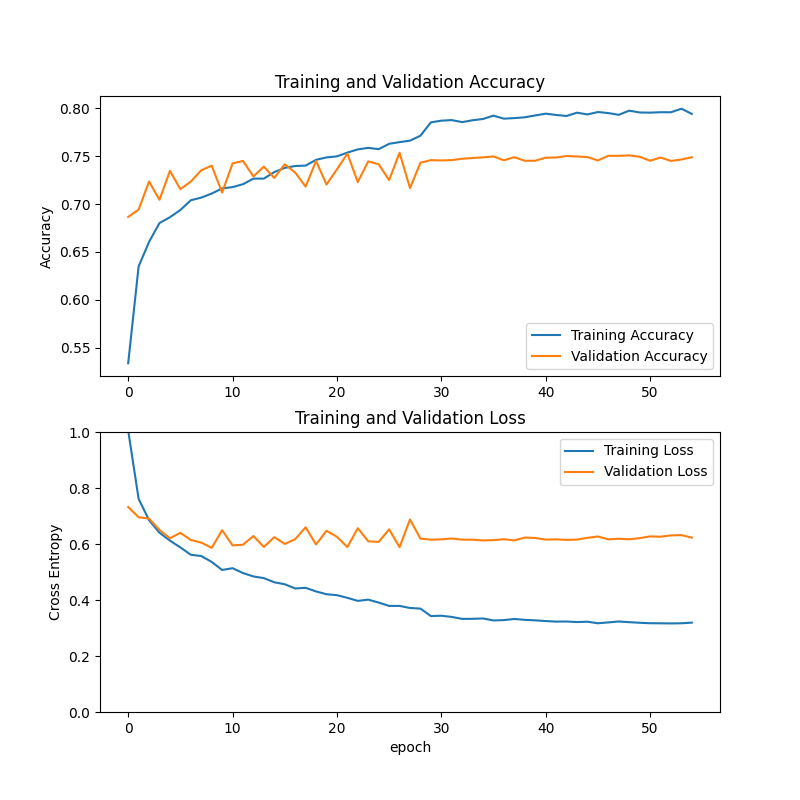
\includegraphics[width=160]{imgs/qualité/cr7/history1.png}
    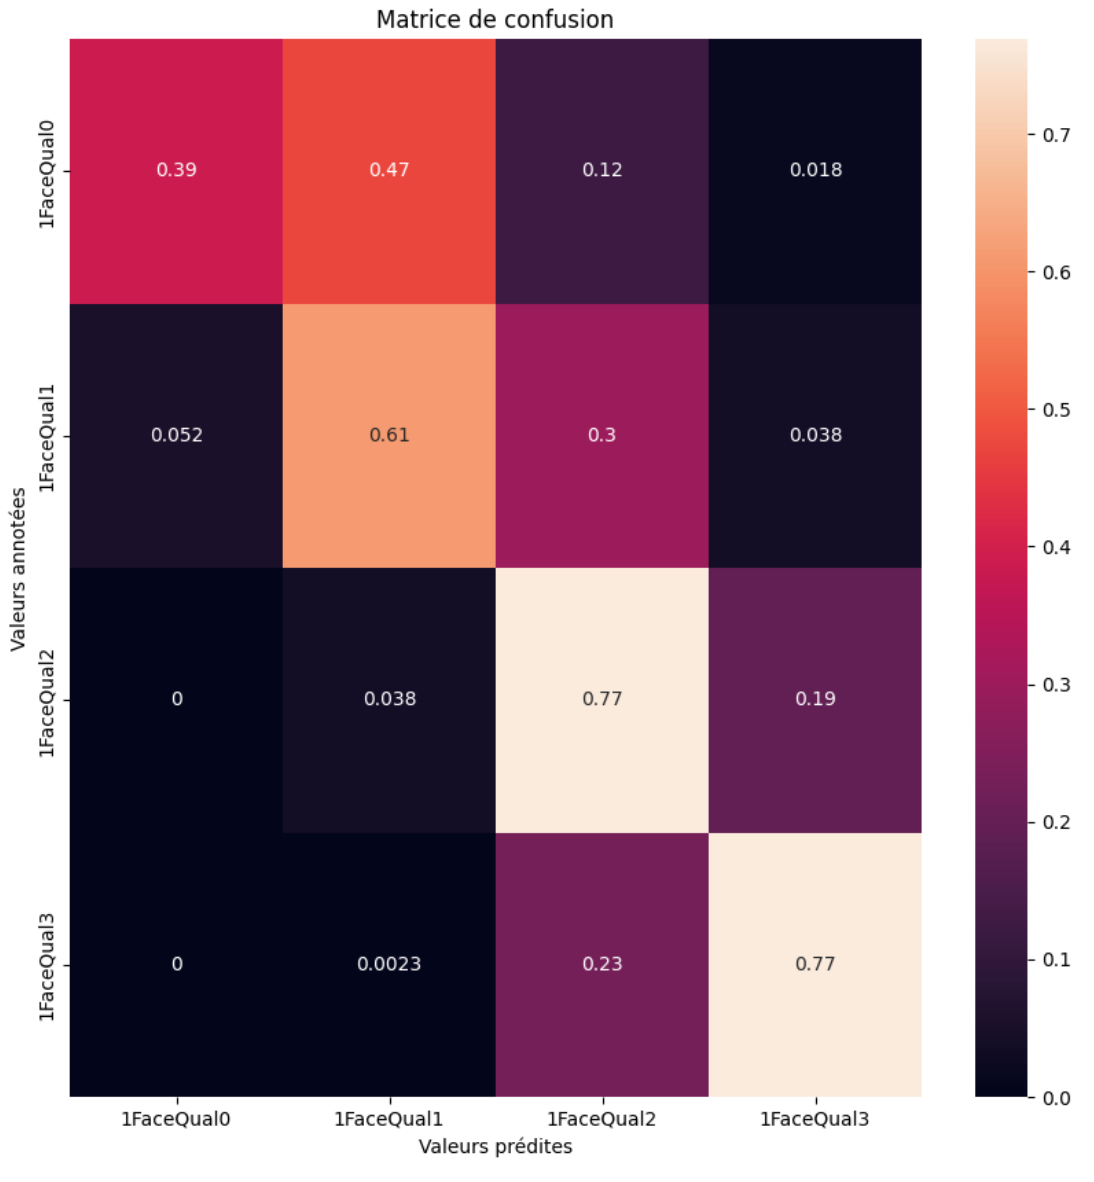
\includegraphics[width=160]{imgs/qualité/cr6/confusion.png}
\end{center}

Pour améliorer ce résultat nous avons rajouté un layer Dropout égal à 0.2 après chaque couche dense (512, puis 256).
\begin{center}
    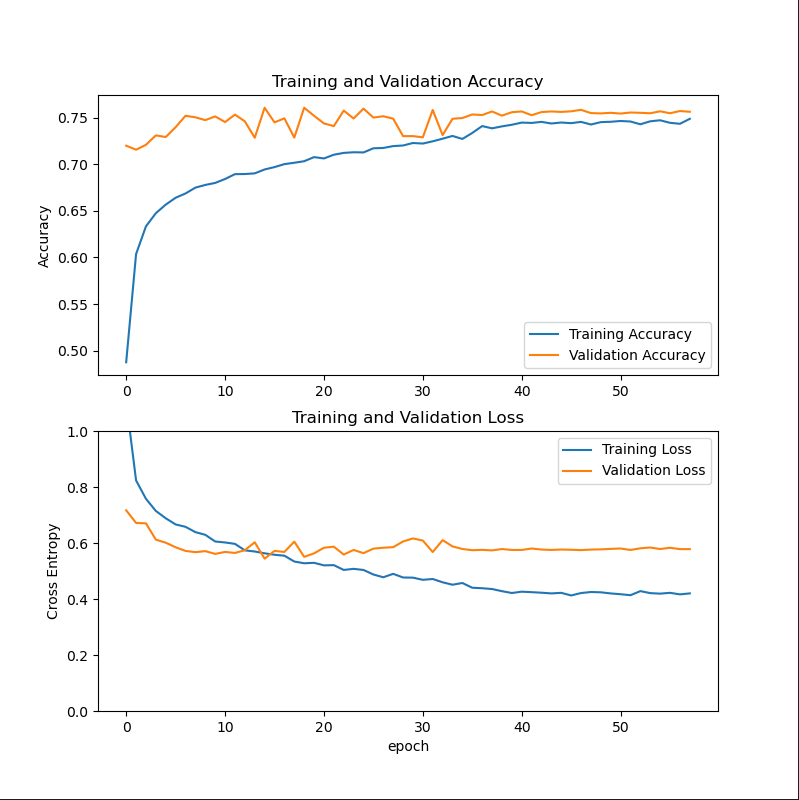
\includegraphics[width=160]{imgs/qualité/cr7/history_drop.png}
    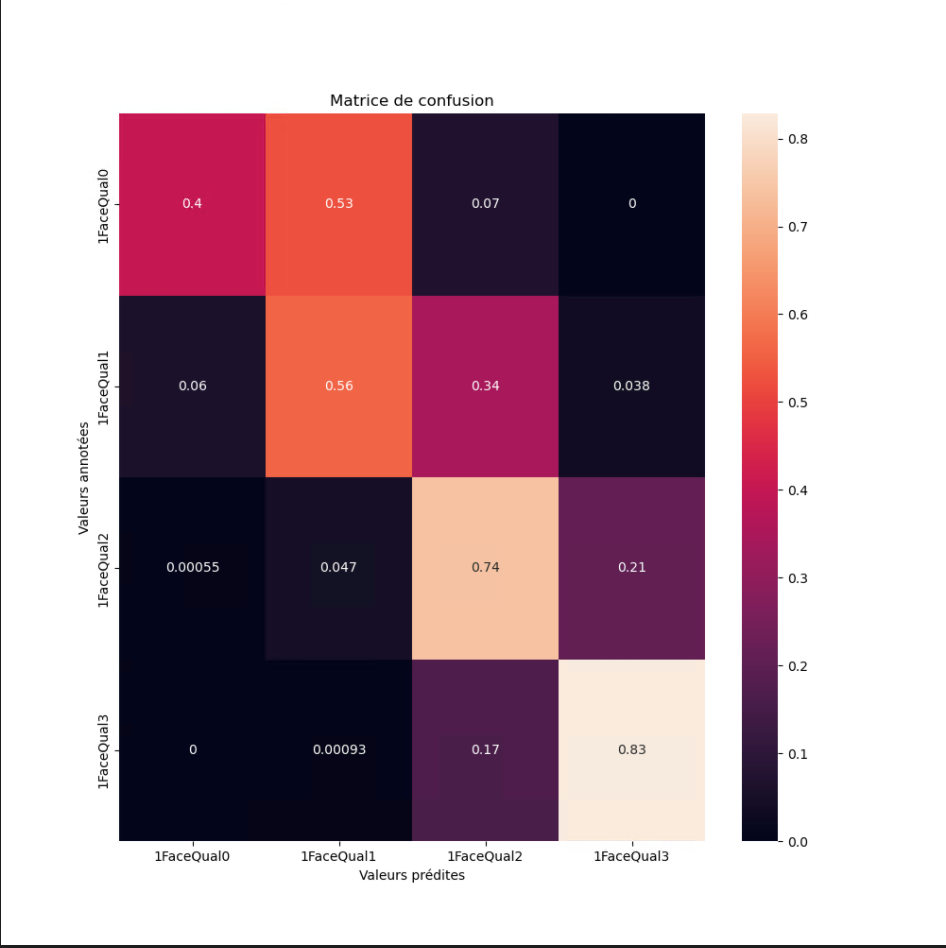
\includegraphics[width=160]{imgs/qualité/cr7/confusion_drop.png}
\end{center}

Le résultat n'est pas bien meilleur, mais le surapprentissage est supprimé. \\

Une autre méthode à explorer pour résoudre un problème de classification multi classe ordonné, est d'utiliser un encodage one-hot particulier tel que décrit sur cette \href{https://stats.stackexchange.com/questions/140061/how-to-set-up-neural-network-to-output-ordinal-data}{réponse} et  \href{https://arxiv.org/pdf/1901.07884.pdf}{papier}.
J'ai donc créé un générateur personnalisé d'images, qui prend des batchs d'images avec leur label et retourne normalement les mêmes batchs avec les mêmes labels encodés sous la nouvelle forme :\\
\begin{gather*}
0 \longrightarrow [0, 0, 0]\ (au\ lieu\ de\ [1, 0, 0, 0])\\
1 \longrightarrow [1, 0, 0]\ (au\ lieu\ de\ [0, 1, 0, 0])\\
2 \longrightarrow [1, 1, 0]\ (au\ lieu\ de\ [0, 0, 1, 0])\\
3 \longrightarrow [1, 1, 1]\ (au\ lieu\ de\ [0, 0, 0, 1])\\
\end{gather*}
Par ailleurs, au lieu d'utiliser une dernière couche à k neurones et pour activation softmax, j'utilise k-1 neurones avec pour activation sigmoid. Enfin, pour avoir le numéro de la classe prédite, on fait la somme des probabilités, ce qui donne par exemple : [1,1,0] \longrightarrow 2
\begin{center}
    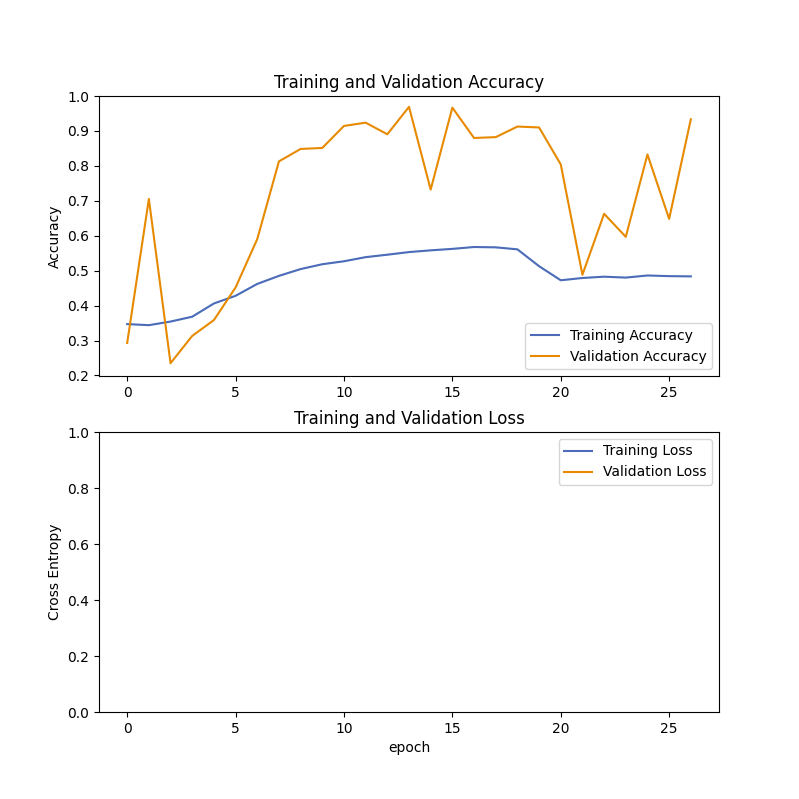
\includegraphics[width=160]{imgs/qualité/cr7/history_hot.png}
    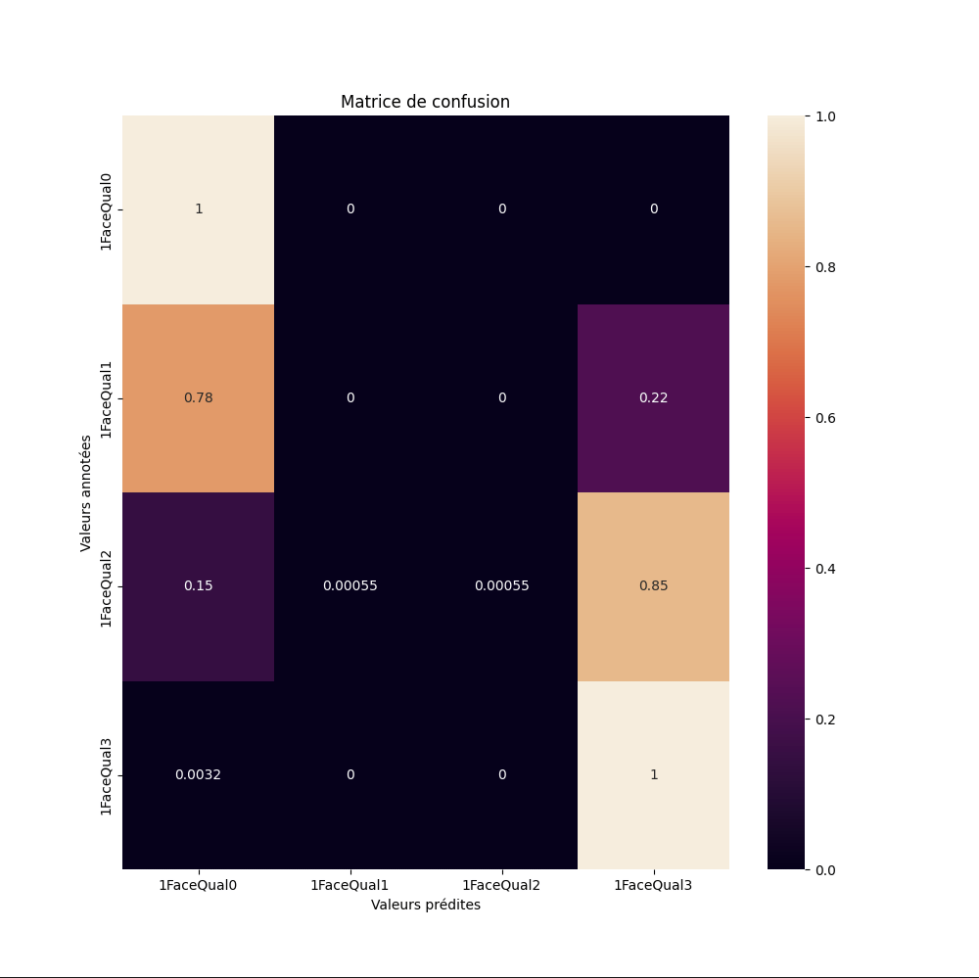
\includegraphics[width=160]{imgs/qualité/cr7/confusion_hot.png}
\end{center}

Clairement, quelque chose ne va pas au niveau du modèle, peut être au niveau de la normalisation ou du préprocessing en one hot. C'est donc sur quoi je travaille actuellement.
Une autre piste qu'il faudra étudier peut être la weighted kappa loss, qui est une fonction de coût qui a pour but également de traiter la classification multiclasse ordonnée : \href{https://www.tensorflow.org/addons/api_docs/python/tfa/losses/WeightedKappaLoss}{WeightedKappaLoss}.


\end{document}
